\documentclass[fleqn]{homework}

\student{Stephen Brennan (smb196)}
\course{}
\assignment{}
\duedate{}

%\usepackage{mathtools}
\usepackage{graphicx}
\usepackage{enumerate}

\begin{document}
  \maketitle

  \begin{problem}{1}
    \begin{question}
      To provide adequate medical service to its constituents at a reasonable
      cost, hospital administrators must constantly seek ways to hold staff
      levels as low as possible while maintaining sufficient staffing to provide
      satisfactory levels of health care.  An urban hospital has three
      departments: the emergency room (department 1), the neonatal intensive
      care nursery (department 2), and the orthopedics (department 3). The
      hospital has three work shifts, each with different levels of necessary
      staffing for nurses. The hospital would like to identify the minimum
      number of nurses required to meet the following three constraints:

      \begin{enumerate}[a.]
      \item The hospital must allocate at least 13, 32, and 22 nurses to the
        three departments over all shifts,
      \item The hospital must assign at least 26, 24, and 19 nurses to the three
        shifts over all departments, and
      \item The minimum and maximum number of nurses allocated to each
        department in a specific shift must satisfy the following limits:

        \begin{tabular}{|l|ccc|}
          \hline
          & Department 1 & Department 2 & Department 3 \\
          \hline
          Shift 1 & (6, 8) & (11, 12) & (7, 12) \\
          Shift 2 & (4, 6) & (11, 12) & (7, 12) \\
          Shift 3 & (2, 4) & (10, 12) & (5, 7) \\
          \hline
        \end{tabular}
      \end{enumerate}

      Suggest a method using maximum flows to identify the minimum number of
      nurses required to satisfy all the constraints.
    \end{question}
  \end{problem}

  \begin{problem}{2}
    \begin{question}
      Formulate the contractor problem (Homework Assignment 1, problem 7) as a
      minimum cost network flow problem, write its dual and complementary
      slackness conditions, and prove that this problem has always an integer
      optimal solution.
    \end{question}
  \end{problem}

  \begin{problem}{3}
    \begin{question}
      Let $G=(V, E)$ be a directed graph with lengths $w(e)$ associated to each
      arc $e\ in E$, and let $s \in V$ be a vertex. Recall that
      $d(v) \le d(u) + w(u,v)$ for $(u,v) \in E$ by linear programming duality,
      where $d(u)$ is the distance of $u \in V$ from $s$. Show that the
      following invariant holds during the execution of Dijkstra’s algorithm: if
      $S$ is the set of permanently labeled nodes and $d(u)$ is the current
      label of vertex $u$, then $d(v) \le d(u) + w(u,v)$ for $(u,v) \in E$,
      $u \in S$, $v \not\in S$.
    \end{question}
  \end{problem}

  \begin{problem}{5}
    \begin{question}
      Apply the successive shortest paths algorithm to the minimum cost flow
      problem in the figure. Show that the algorithm performs eight
      augmentations of unit flow and that their cost (i.e., the sum of the arc
      costs in the path in the residual network) is 0, 1, 2, 3, 4, 5, and 6.

      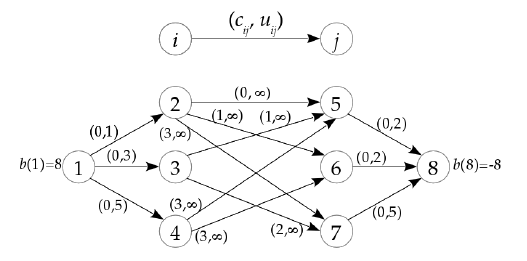
\includegraphics[width=0.6\textwidth]{p5-fig.png}
    \end{question}
  \end{problem}

  \begin{problem}{7}
    \begin{question}
      Consider the following practical improvement of the successive shortest
      path algorithm:

      \begin{enumerate}[a.]
      \item Terminate the execution of Dijkstra's algorithm whenever it
        permanently labels a deficit node $v$, and

      \item Modify the node potentials by setting $\pi(u)$ to $\pi(u)-d(u)$ if
        node $u$ is permanently labelled and by setting $\pi(u)$ to
        $\pi(u)-d(v)$ if node $u$ is temporarily labelled.
      \end{enumerate}

      Show that after the algorithm has updated the node potentials in this
      manner, all the arcs in the residual network have non-negative reduced
      costs and that all arcs in the shortest path from node $k$ to node $v$
      have zero reduced cost. Use the statement of problem 3.
    \end{question}
  \end{problem}

\end{document}